\chapter{Quantum Entanglements, Part 1}

These notes follow Leonard Susskind's second lecture in the supplementary \emph{Quantum Entanglement} track, in an edition curated by LazyingArt LLC. The lecture opens by leaving the world of classical bits and entering quantum mechanics at its simplest nontrivial point: a single electron spin. But it does not begin with formalism. It begins with a puzzle. The electron can be prepared as though it were pointing in many different directions, yet an up-down measurement returns only two answers. The chapter should be read in that order. We first let the classical picture build up enough force to fail, and only then do we introduce the complex vector space of states that can carry the physics.

\section{Classical Bits, Qubits, and the Spin Example}

We begin where the lecture begins: classical physics with a discrete state space. In that setting the space of states is a Boolean space, a collection of points, one point for each possible state, and the logic governing those states is ordinary classical logic. A classical bit is the simplest example. It has two possible values and nothing in between.

If we draw a two-state object with one end distinguished from the other, then ``up'' is one state and ``down'' is another. That is a classical bit in its barest form: two possibilities, no intermediate state. One can build many-bit systems out of such objects, and in classical physics that point of view goes a surprisingly long way.

Quantum mechanics forces a different notion of state, and Susskind chooses the simplest example immediately: the spin of an electron. He also warns us, at the outset, that the word \emph{vector} is about to become dangerous.

On the one hand, there is the familiar vector in ordinary space: an arrow with magnitude and direction. To keep the distinction visible, we will call that a \emph{spatial vector}. The electron carries such a spatial vector in the form of its magnetic moment. The magnetic moment has a fixed magnitude for every electron, but its direction may vary.

On the other hand, there is the abstract vector that belongs to a vector space of states. That vector is not an arrow in space. It is a mathematical object, and before long it will be this abstract vector, not the spatial arrow, that carries the state of the qubit.

That is already the lecture's first tension. The electron seems to come equipped with something that can point in any direction in space, but the measurement story we are heading toward will not return a continuum of answers. We are being steered toward a conflict between classical imagery and quantum logic.

\section{The Classical Preparation-and-Detection Story, and Why It Fails}

Susskind next does something very deliberate: he tells a classical story in full. He even says that for the moment we are still thinking very classically. The point is not to endorse that story. The point is to let it fail in a way that makes the quantum alternative unavoidable.

Imagine the electron as a tiny bar magnet with a north pole and a south pole. Suppose we place it in a strong external magnetic field. A classical magnet does not, in general, jump instantly into alignment. In vacuum, with no friction, it precesses around the external field. Then it radiates away its excess energy and settles into the energetically preferred orientation. That is the lecture's classical picture of \emph{preparation}: choose the direction of the external field, wait long enough, and the electron's magnetic moment comes into equilibrium with that field.

The same setup then suggests a classical model of \emph{detection}. Put the electron into a known field and watch how much radiation it emits as it relaxes. If the electron begins almost aligned with the field, only a little energy is emitted. If it begins farther away, more energy is emitted. If it begins anti-aligned, the emitted energy is maximal. So, classically, the emitted energy should be a continuous function of the initial angle.

The lecture's experimental staging is captured well enough by a schematic reconstruction:

\begin{figure}[h]
\centering
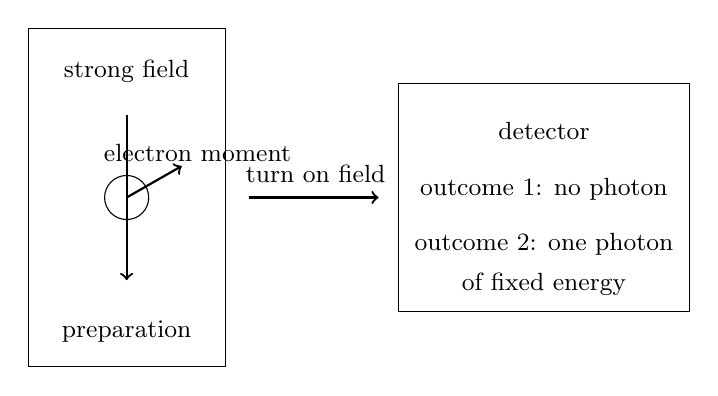
\begin{tikzpicture}[scale=1.0]
\draw (-0.2,0) rectangle (2.3,4.3);
\draw (1.05,3.75) node {\small strong field};
\draw[thick,->] (1.05,3.2) -- (1.05,1.1);
\draw (1.05,2.15) circle (0.28);
\draw[thick,->] (1.05,2.15) -- (1.75,2.55);
\draw (1.95,2.72) node {\small electron moment};
\draw (1.05,0.45) node {\small preparation};

\draw (4.5,0.7) rectangle (8.2,3.6);
\draw (6.35,3.0) node {\small detector};
\draw (6.35,2.25) node {\small outcome 1: no photon};
\draw (6.35,1.55) node {\small outcome 2: one photon};
\draw (6.35,1.05) node {\small of fixed energy};
\draw[thick,->] (2.6,2.15) -- (4.25,2.15);
\draw (3.45,2.45) node {\small turn on field};
\end{tikzpicture}
\end{figure}

In this classical picture we do \emph{not} need an explicit formula for emitted energy as a function of angle, and the lecture never gives one. What matters is only the qualitative statement that the response is continuous.

\begin{figure}[h]
\centering
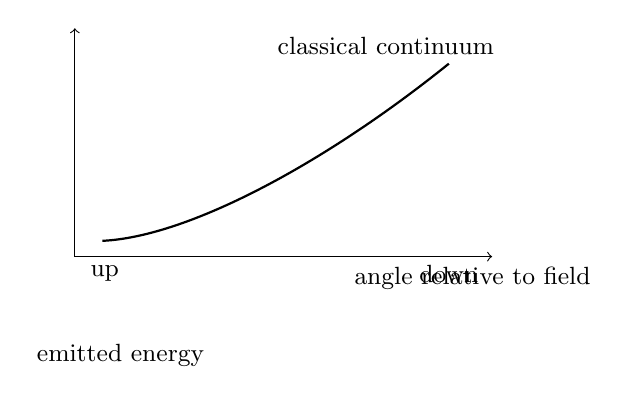
\begin{tikzpicture}[scale=1.0]
\draw[->] (0,0) -- (5.3,0);
\draw[->] (0,0) -- (0,2.9);
\draw (5.05,-0.28) node {\small angle relative to field};
\draw[rotate=90] (-1.25,-0.58) node {\small emitted energy};
\draw[thick] (0.35,0.2) .. controls (1.45,0.25) and (3.2,1.2) .. (4.75,2.45);
\draw (0.38,-0.22) node {\small up};
\draw (4.75,-0.22) node {\small down};
\draw (3.95,2.68) node {\small classical continuum};
\end{tikzpicture}
\end{figure}

This, however, is exactly the point at which the lecture reverses itself. Susskind says, in effect: that was the wrong story. For a real electron the detector does \emph{not} produce a continuous output.

Once the magnetic field is turned on, only two things can happen:
\begin{itemize}
\item no photon is emitted;
\item one photon of a definite energy is emitted, namely the energy corresponding to the transition from down to up.
\end{itemize}

Nothing in between ever appears. The detector does not report a small amount of up or a medium amount of down. It returns one of two answers.

What \emph{does} depend on the preparation is the probability distribution over those two answers. If the electron has been prepared vertically upward and we measure it in the same up-down setup, then no photon is emitted. If it has been prepared vertically downward and we reverse the field appropriately, the photon is emitted with probability one. If it has been prepared horizontally and then measured in the vertical device, the two outcomes occur with equal probabilities:
\begin{equation}
P(\text{one photon})=\frac{1}{2},
\qquad
P(\text{no photon})=\frac{1}{2}.
\end{equation}

The lecture also pauses, in audience questions, over the operational meaning of this probability. A single run does not display a distribution. We must repeat the whole prepare-and-measure procedure many times. And once a given measurement has found the electron in the up state, repeating the same measurement does not recover the earlier preparation. The system has been fixed relative to that detector.

\subsection{Question \& Answer}

\paragraph{Question.} If the electron can be prepared in arbitrary directions, why does the up-down detector return only up or down?

\paragraph{Answer.} Because the preparation direction does not create new outcomes for a fixed detector. A vertical detector always asks a binary question. The preparation changes only the probabilities of the two available answers. The mystery, then, is not that new detector values appear. The mystery is that a continuously variable preparation changes only a two-valued probability distribution.

That is the lecture's main puzzle. In one sense the electron seems to have only two measurable states. In another sense it can still be prepared in many directions. A set of two points will not be enough to describe such an object.

\section{From the Puzzle to a Complex Vector Space of States}

Now comes the lecture's central pivot. Susskind says, in substance, that we need a different mathematics of states. Not a Boolean set of two points, but a vector space.

He also tells us what the bargain is. We are going to do some abstract mathematics first and interpret it afterward. The first piece of that mathematics is the algebra of complex numbers.

We introduce the imaginary unit \(i\) by
\begin{equation}
i^2=-1.
\end{equation}
A complex number is written
\begin{equation}
z=a+ib,
\qquad
z^*=a-ib,
\end{equation}
where \(a\) and \(b\) are real and \(z^*\) denotes the complex conjugate.

The lecture's blackboard cluster for this interlude is worth keeping, even though the frame is only partial evidence for the exact line-by-line algebra.

\begin{figure}[h]
\centering

\includegraphics[width=0.58\textwidth]{lecture_02_figure_02.png}
\end{figure}

A key example is the product of a complex number with its conjugate:
\begin{align}
z^*z
&=(a+ib)(a-ib) \\
&=a^2-iab+iab+b^2 \\
&=a^2+b^2.
\end{align}
The cross terms cancel, and the result is real and nonnegative. That is not yet quantum mechanics, but it is the algebraic pattern quantum mechanics will use when amplitudes become probabilities.

\begin{definition}
A complex vector space, in the minimal sense used in this lecture, is a collection of objects that can be added and multiplied by complex numbers, with the result remaining in the same collection.
\end{definition}

The lecture then gives the simplest concrete realization of this idea: column vectors with complex entries. If
\[
A \leftrightarrow \begin{pmatrix}A_1\\A_2\\A_3\end{pmatrix},
\]
then multiplication by a complex number \(c\) is defined componentwise:
\begin{equation}
c\begin{pmatrix}A_1\\A_2\\A_3\end{pmatrix}
=
\begin{pmatrix}cA_1\\cA_2\\cA_3\end{pmatrix},
\end{equation}
and addition is defined by
\begin{equation}
\begin{pmatrix}A_1\\A_2\\A_3\end{pmatrix}
+
\begin{pmatrix}B_1\\B_2\\B_3\end{pmatrix}
=
\begin{pmatrix}A_1+B_1\\A_2+B_2\\A_3+B_3\end{pmatrix}.
\end{equation}

There is no need yet to say more. The point is to establish the kind of space in which quantum states will live. For the spin of a single electron, the relevant case will be a two-dimensional complex vector space.

\section{Column Vectors, Bras, Kets, and the Inner Product}

The lecture now tightens the notation. Abstract vectors are represented by columns, and their conjugates by rows.

If
\[
|a\rangle \leftrightarrow \begin{pmatrix}a_1\\a_2\end{pmatrix},
\]
then its conjugate is represented by
\[
\langle a| \leftrightarrow \begin{pmatrix}a_1^* & a_2^*\end{pmatrix}.
\]
The star is implicit in turning the ket into the bra; that is exactly the point Susskind pauses over in the lecture.

The notation \(\langle b|a\rangle\) is a \emph{bracket} split into its two halves, bra and ket. In components the rule is
\begin{equation}
\langle b|a\rangle = b_1^*a_1+b_2^*a_2.
\end{equation}
This is the inner product.

If we take the inner product of a vector with itself, we find
\begin{equation}
\langle a|a\rangle = a_1^*a_1+a_2^*a_2.
\end{equation}
Each term has the form \(z^*z\), and therefore each term is real and nonnegative. So \(\langle a|a\rangle\) itself is real and nonnegative.

\begin{remark}
The lecture interprets \(\langle a|a\rangle\) as the square of the size of the vector. We are not yet using this abstractly; we are preparing it for a physical interpretation.
\end{remark}

This is the point at which the mathematics begins to justify itself. Complex numbers were introduced because their conjugation law produces positive real quantities. Those are exactly the quantities that can later be interpreted as probabilities.

\section{Up and Down as an Orthogonal Basis of States}

At this point Susskind explicitly returns from the abstract vector space to the quantum bit. The detector has two possible outputs. Let us denote the corresponding states by
\[
|+\rangle
\qquad \text{and} \qquad
|-\rangle.
\]
These stand for the electron being found up or down in the chosen measurement basis.

Now the lecture makes the space concrete. A general state of the electron spin is written as a linear combination
\begin{equation}
|\psi\rangle=a_+|+\rangle+a_-|-\rangle.
\end{equation}
The corresponding blackboard layout is an important piece of visual evidence because it shows exactly how the coefficient-weighted basis states are assembled into a single column vector.

\begin{figure}[h]
\centering

\includegraphics[width=0.68\textwidth]{lecture_02_figure_03.png}
\end{figure}

Once the basis has been fixed, the canonical column-vector representatives are
\begin{equation}
|+\rangle \leftrightarrow \begin{pmatrix}1\\0\end{pmatrix},
\qquad
|-\rangle \leftrightarrow \begin{pmatrix}0\\1\end{pmatrix}.
\end{equation}
Then
\[
a_+|+\rangle \leftrightarrow \begin{pmatrix}a_+\\0\end{pmatrix},
\qquad
a_-|-\rangle \leftrightarrow \begin{pmatrix}0\\a_-\end{pmatrix},
\]
and adding these two contributions gives
\begin{equation}
|\psi\rangle \leftrightarrow \begin{pmatrix}a_+\\a_-\end{pmatrix}.
\end{equation}

The lecture later revisits the same identification more cleanly on the board, and that cleaner basis-fixing picture should remain visible as well.

\begin{figure}[h]
\centering

\includegraphics[width=0.62\textwidth]{lecture_02_figure_04.png}
\end{figure}

Now comes the physical interpretation. The squared magnitudes of the coefficients are the probabilities for the two detector outcomes:
\begin{equation}
P(+)=a_+^*a_+=|a_+|^2,
\qquad
P(-)=a_-^*a_-=|a_-|^2.
\end{equation}
Since these are the only two possibilities, they must add to one:
\begin{equation}
|a_+|^2+|a_-|^2=1.
\end{equation}
Equivalently,
\begin{equation}
\langle \psi|\psi\rangle=1.
\end{equation}
This is the normalization condition. The physical states are the normalized vectors in the vector space.

The two basis states are orthonormal:
\begin{align}
\langle +|+\rangle &= 1, &
\langle -|-\rangle &= 1, \\
\langle +|-\rangle &= 0, &
\langle -|+\rangle &= 0.
\end{align}
The lecture explicitly checks these relations in components. For example,
\[
\langle +|-\rangle
=
\begin{pmatrix}1 & 0\end{pmatrix}
\begin{pmatrix}0\\1\end{pmatrix}
=0.
\]
So the up and down states correspond to orthogonal vectors in the state space.

\paragraph{Worked example.}
The lecture does not move too quickly past its first nontrivial example. It writes, in effect,
\[
\begin{pmatrix}1\\1\end{pmatrix},
\]
then immediately notices that this cannot yet be a physical state because its norm-squared is \(2\). To repair it, we divide by \(\sqrt{2}\):
\begin{equation}
\frac{1}{\sqrt{2}}\begin{pmatrix}1\\1\end{pmatrix}.
\end{equation}
Now the probabilities are
\[
P(+)=\frac{1}{2},
\qquad
P(-)=\frac{1}{2}.
\]
This is the lecture's equal-weight state. It is not pure up and not pure down. It is one of the states associated with a horizontal preparation.

We now see how the lecture wants us to think. A detector aligned along a chosen axis still returns only two answers. But the state space is larger than those two detector values, because it contains all normalized linear combinations of the corresponding basis vectors.

\section{What the State Vector Does and Does Not Encode}

After the break Susskind performs a reset. More than one person is probably confused, he says, about the two notions of vector. That is exactly the right place to slow down and separate them.

A spatial vector in ordinary space has three real components. A two-component state vector,
\[
\begin{pmatrix}a_+\\a_-\end{pmatrix},
\]
has two complex components, which means four real numbers before any constraints are imposed. So the state vector is not just a disguised spatial arrow.

Of course, not all four of those real numbers are physically independent. Normalization removes one. Overall phase removes another. But the lecture does not yet build the full geometry that connects state vectors to spatial directions, and we should not force it. The right statement, and the lecture's own statement, is simpler: the two objects are related, but not simply related.

There is another important clarification here. The dimension of the state space is fixed experimentally. The up-down measurement has two possible outcomes, and that is why we use a two-dimensional complex vector space. In that sense the mathematics is not arbitrary. The experiment tells us how many basis states we need.

\subsection{Question \& Answer}

\paragraph{Question.} Is \(-|+\rangle\) the same thing as \(|-\rangle\)?

\paragraph{Answer.} No. The symbol \(-\) in \(|-\rangle\) is part of a label. It does not mean minus one times the plus state. By contrast, \(-|+\rangle\) is an ordinary scalar multiple of \(|+\rangle\), and it is perfectly allowed in the vector space.

This answer leads immediately to the lecture's next point. The states \(|+\rangle\) and \(-|+\rangle\) are not equal as vectors, but they represent the same physics, because an overall phase does not change the probabilities of any measurement. More generally, if \(|\psi\rangle\) is multiplied by a complex number of magnitude one, the physical state is unchanged.

But a relative sign inside a superposition is a different matter. The states
\[
a_+|+\rangle+a_-|-\rangle
\qquad \text{and} \qquad
a_+|+\rangle-a_-|-\rangle
\]
need not represent the same physics. The lecture does not yet unpack the full meaning of relative phase, but it clearly insists on this distinction: overall phase is inessential, relative phase can matter.

\section{From Classical Observables to Quantum Matrices}

The lecture now shifts its center of gravity. Up to now we have been asking what a state is. Next we ask what a measurable quantity is.

In classical mechanics, if the possible states are discrete points labeled by \(n\), then an observable is simply a function that assigns a real number to each state:
\[
f_n.
\]
If the system is not known exactly, but only through a probability distribution \(p_n\), then the average value of the observable over many repeated experiments is
\begin{equation}
\langle f\rangle=\sum_n p_n f_n.
\end{equation}

The lecture lingers here because it wants matrices to emerge by motivation rather than fiat. A coin provides the simplest example. Suppose heads is assigned the value \(+1\) and tails the value \(-1\). If the probabilities are \(p_+\) and \(p_-\), then
\begin{equation}
\langle f\rangle=p_+-p_-.
\end{equation}
This is the average value of the observable, not necessarily an attainable single-shot outcome.

\subsection{Question \& Answer}

\paragraph{Question.} How can the average value be zero when zero is not one of the actual outcomes?

\paragraph{Answer.} Because the average value is not the same thing as a detector reading from a single run. If a fair coin yields \(+1\) half the time and \(-1\) half the time, then the average over many trials is zero, even though no single toss ever produces zero. The average is a summary of the distribution, not a new observable value that occurs in one trial.

The lecture then singles out a special classical observable: the indicator function that is \(1\) on one state and \(0\) on all the others. In that case the average is exactly the probability of that state. So if we know how to compute average values of all observables, we also know how to recover probabilities.

This now raises the quantum question: what mathematical objects represent observables in quantum mechanics? The answer, for the present finite-dimensional setting, is matrices.

A matrix acts on a state vector and produces another vector:
\begin{equation}
M|a\rangle=|a'\rangle.
\end{equation}
The lecture's board picture should remain in place here because it preserves the two-level transition from abstract operator language to explicit component calculation.

\begin{figure}[h]
\centering

\includegraphics[width=0.66\textwidth]{lecture_02_figure_05.png}
\end{figure}

If
\[
M=\begin{pmatrix}m_{11}&m_{12}\\m_{21}&m_{22}\end{pmatrix},
\qquad
|a\rangle=\begin{pmatrix}a_1\\a_2\end{pmatrix},
\]
then the component rule is
\begin{equation}
\begin{pmatrix}
m_{11} & m_{12} \\
m_{21} & m_{22}
\end{pmatrix}
\begin{pmatrix}
a_1 \\
a_2
\end{pmatrix}
=
\begin{pmatrix}
m_{11}a_1+m_{12}a_2 \\
m_{21}a_1+m_{22}a_2
\end{pmatrix}.
\end{equation}

Susskind first motivates this by going back to a very ordinary real vector space, the plane of arrows drawn on the board. In that setting matrices represent linear transformations:
\begin{itemize}
\item
\[
\begin{pmatrix}
2 & 0 \\
0 & 2
\end{pmatrix}
\]
doubles every vector;

\item
\[
\begin{pmatrix}
1 & 0 \\
0 & 2
\end{pmatrix}
\]
stretches only the \(y\)-component;

\item
\[
\begin{pmatrix}
0 & 1 \\
1 & 0
\end{pmatrix}
\]
reflects across the diagonal \(x=y\);

\item
\[
\begin{pmatrix}
0 & 1 \\
-1 & 0
\end{pmatrix}
\]
rotates the plane by \(90^\circ\), in the clockwise convention used in the discussion.
\end{itemize}

The lesson is simple: matrices are the language of linear transformations of vector spaces. That is why they are the right candidates for quantum observables.

Now comes the special class singled out by the lecture.

\begin{definition}
A matrix \(M\) is Hermitian if
\begin{equation}
M_{ij}=M_{ji}^*.
\end{equation}
\end{definition}

This is a kind of reality condition, though it does \emph{not} say that every entry is real. It says, first, that on the diagonal
\[
M_{ii}=M_{ii}^*,
\]
so diagonal entries are real. It says, second, that off-diagonal entries come in complex-conjugate pairs. In the special case that all entries are real, Hermitian reduces to symmetric.

The lecture ends this part of the story with a clear declaration. In classical mechanics observables are functions on state points. In quantum mechanics observables will be represented by Hermitian operators, which at the moment means Hermitian matrices.

There is one further preview. If we want to \emph{kick} the electron, that is not generally done by a Hermitian operator. It is done by a unitary operator. At this stage only one fact is stated: unitary operators preserve the length of vectors. Their role in dynamics and physical operations belongs to what comes next.

\section{Summary}

The lecture has carried us from a concrete spin-measurement puzzle to the threshold of the quantum formalism. We began with a classical bit and a classical magnetic-arrow picture of the electron. We let that picture generate a continuous detector response, and then watched the lecture reject it. A real electron, measured in a fixed up-down setup, yields only two outcomes. What varies with preparation is not the list of outcomes but the probability distribution over them.

That failure of the classical story forced a new mathematics of states. We introduced complex numbers, conjugation, column vectors, bras, kets, and the inner product. We chose the orthonormal basis \(|+\rangle\) and \(|-\rangle\), wrote a general qubit state as
\[
|\psi\rangle=a_+|+\rangle+a_-|-\rangle,
\]
and interpreted \(|a_+|^2\) and \(|a_-|^2\) as probabilities, subject to normalization.

After that, the lecture shifted from states to observables. Classical observables are functions \(f_n\) on discrete states, with averages
\[
\langle f\rangle=\sum_n p_n f_n.
\]
Quantum observables are more intricate: they are represented by matrices acting on state vectors, with Hermitian matrices singled out as the measurable ones. That is the mathematical entrance fee the lecture insists upon before entanglement can be discussed honestly. Once states, inner products, and Hermitian operators are in hand, the rest of the structure of quantum mechanics can be built without sleight of hand.